\appchapter{Implementations Experiments}
\label{appendix:experiments:implementations}

% SECTION START %
\section{Parallel Implementations (Best Runtimes)}
\begin{figure}[H]
\begin{adjustwidth}{-2cm}{-2cm}
\centering
\begin{subfigure}{.62\textwidth}
    \centering
    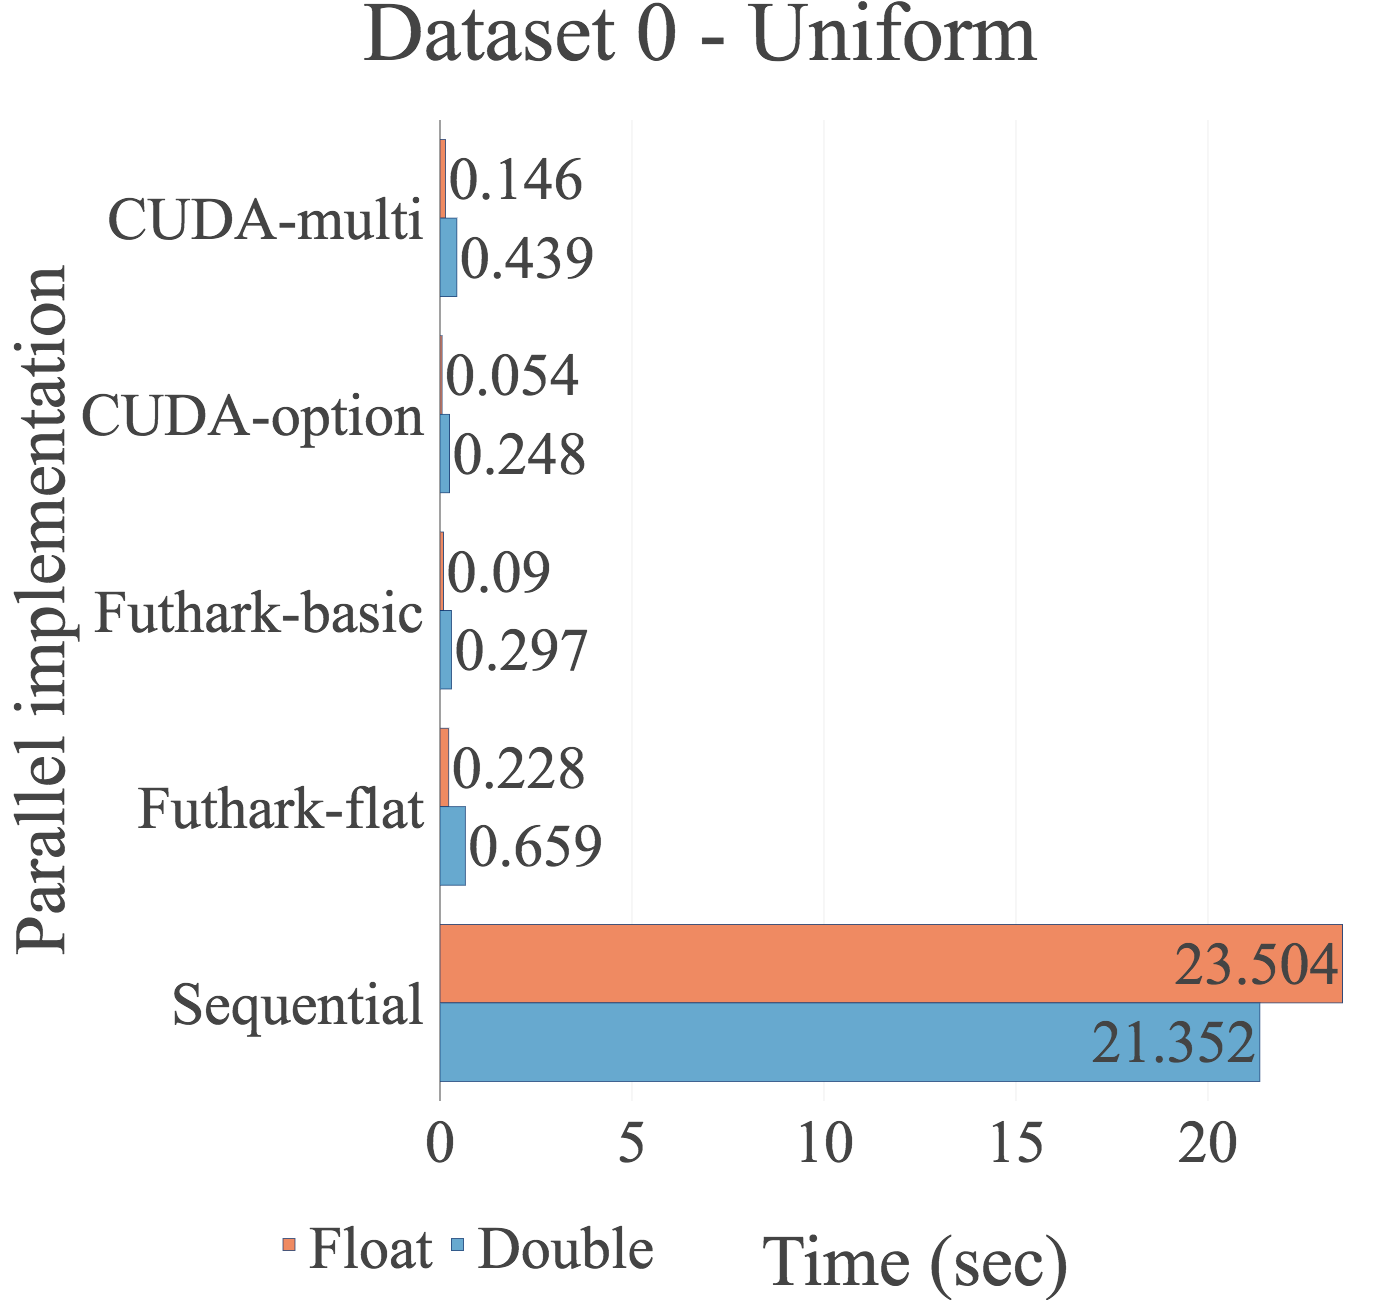
\includegraphics[width=1\textwidth]{img/experiments/all-approaches-0_UNIFORM.png}
\end{subfigure}
\begin{subfigure}{.62\textwidth}
    \centering
    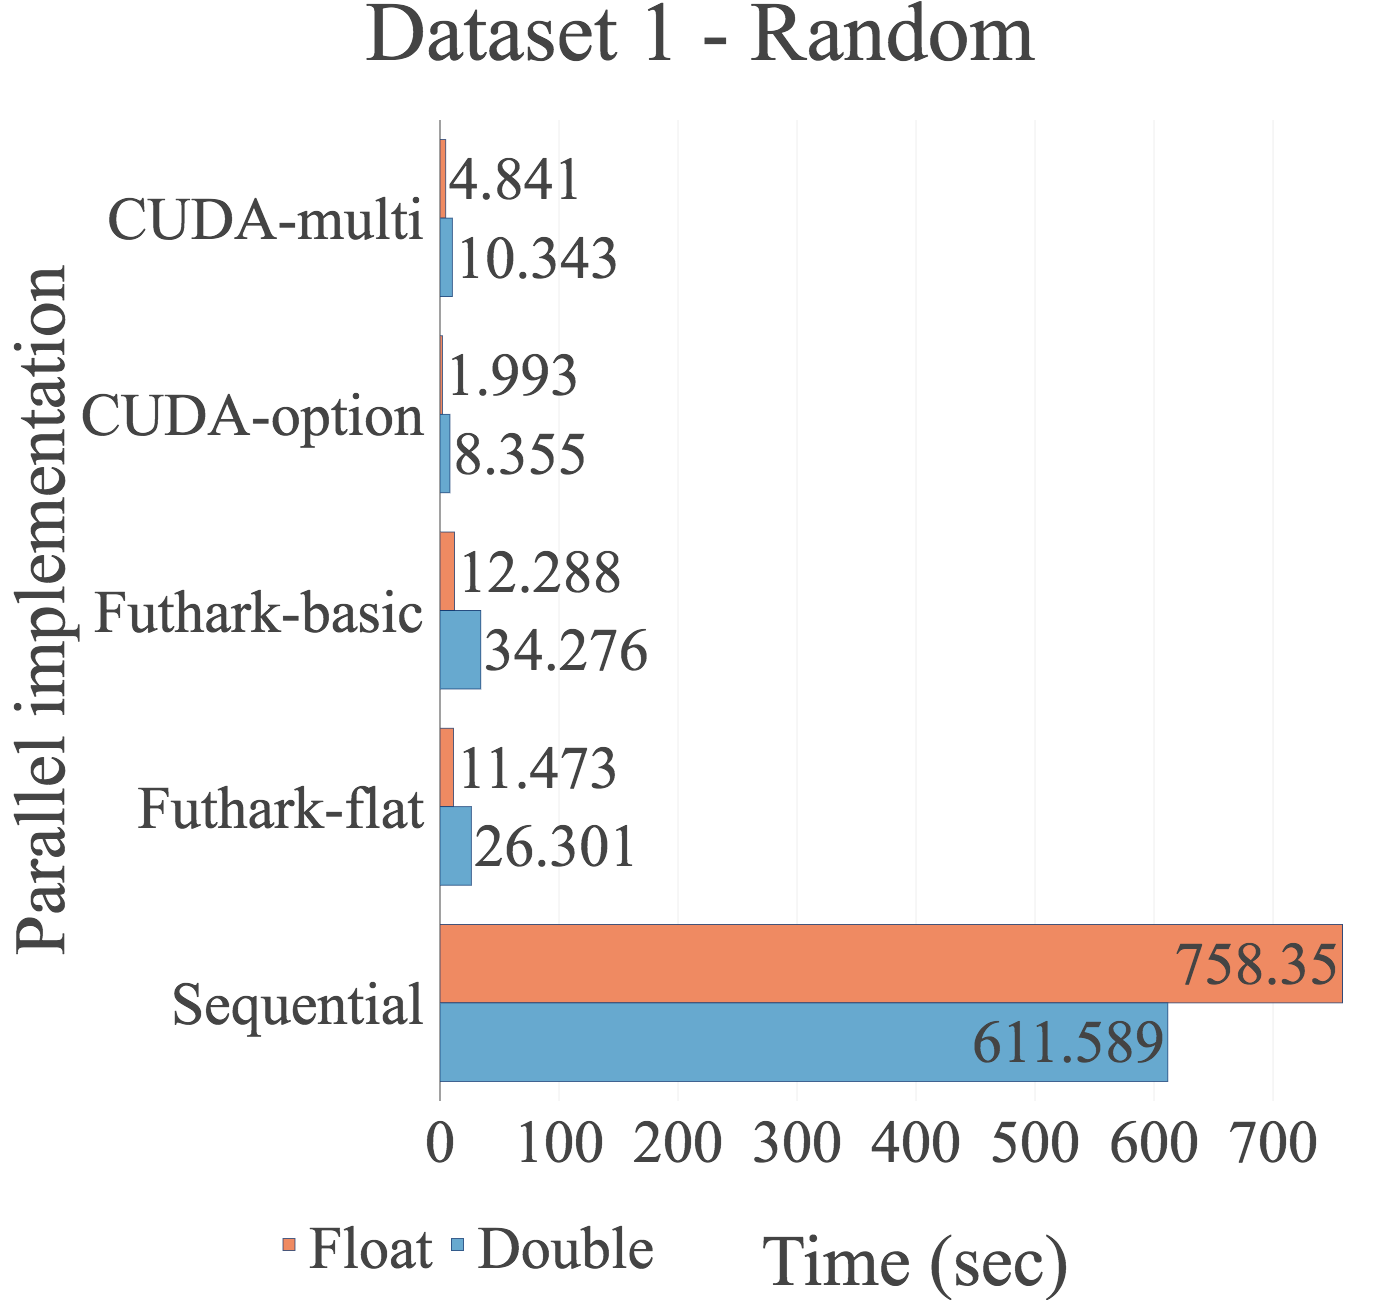
\includegraphics[width=1\textwidth]{img/experiments/all-approaches-1_RAND.png}
\end{subfigure}
\par\bigskip
\par\bigskip
\begin{subfigure}{.62\textwidth}
  \centering
  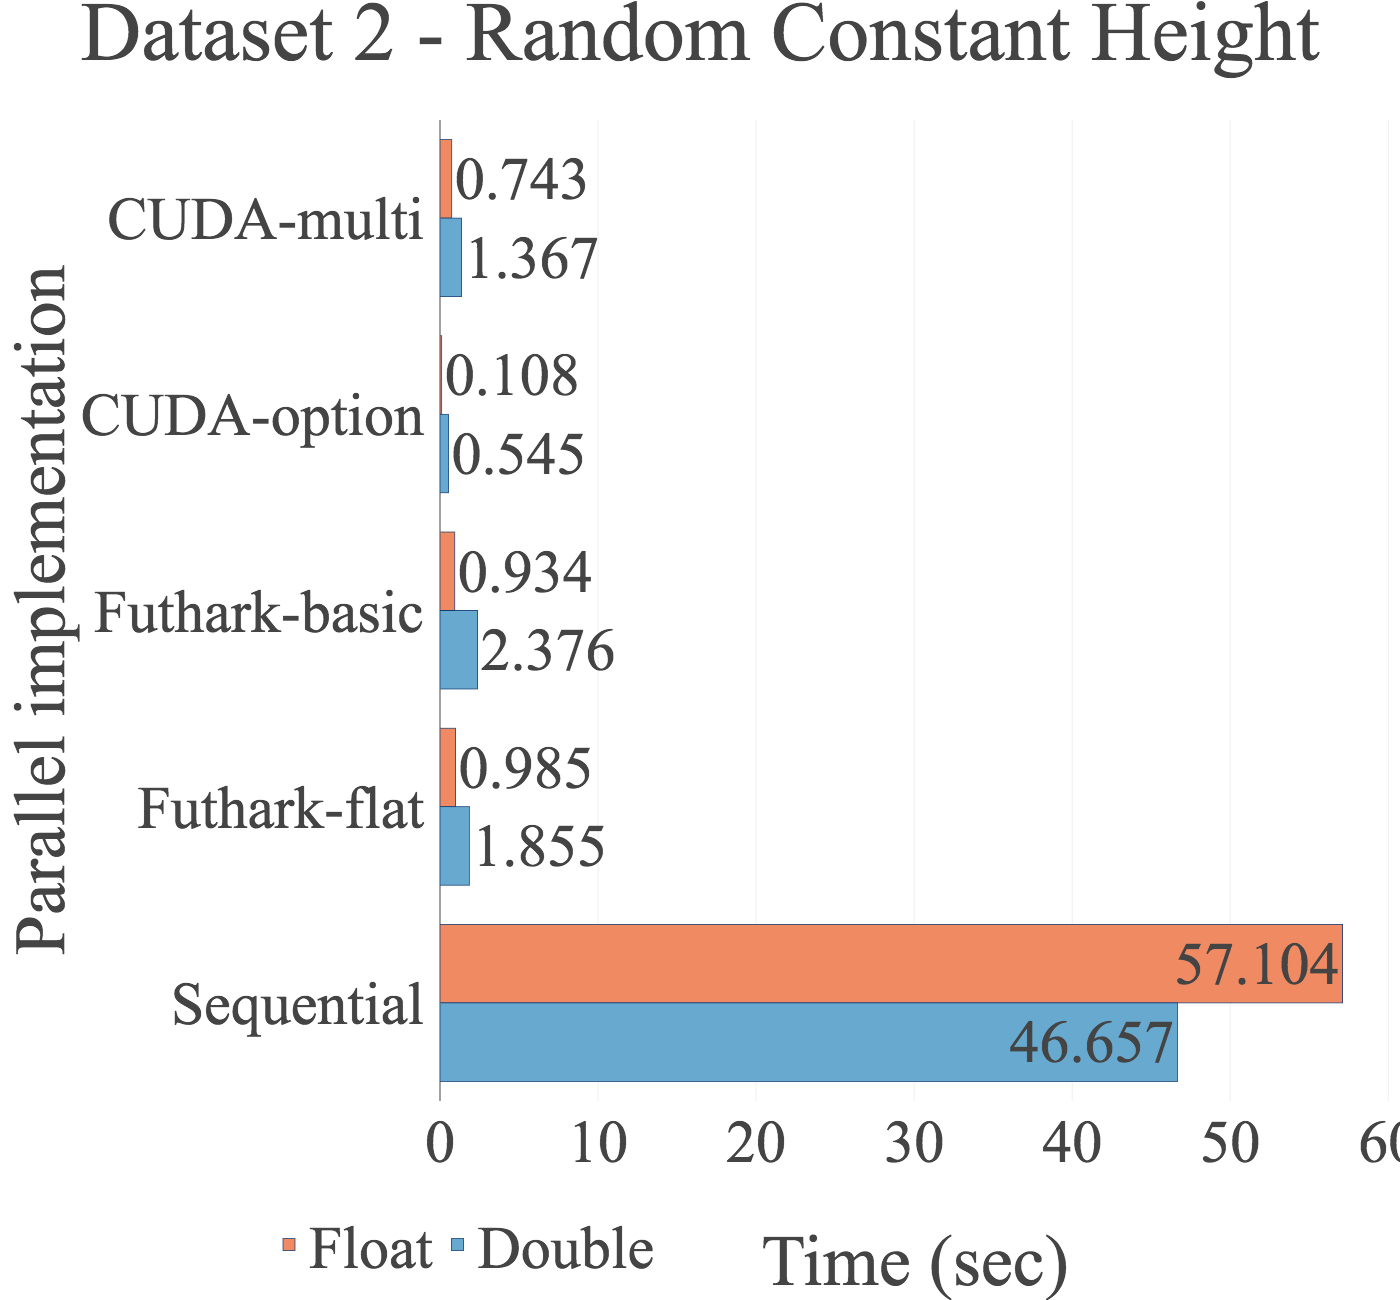
\includegraphics[width=1\textwidth]{img/experiments/all-approaches-2_RANDCONSTHEIGHT.png}
\end{subfigure}
\begin{subfigure}{.62\textwidth}
  \centering
  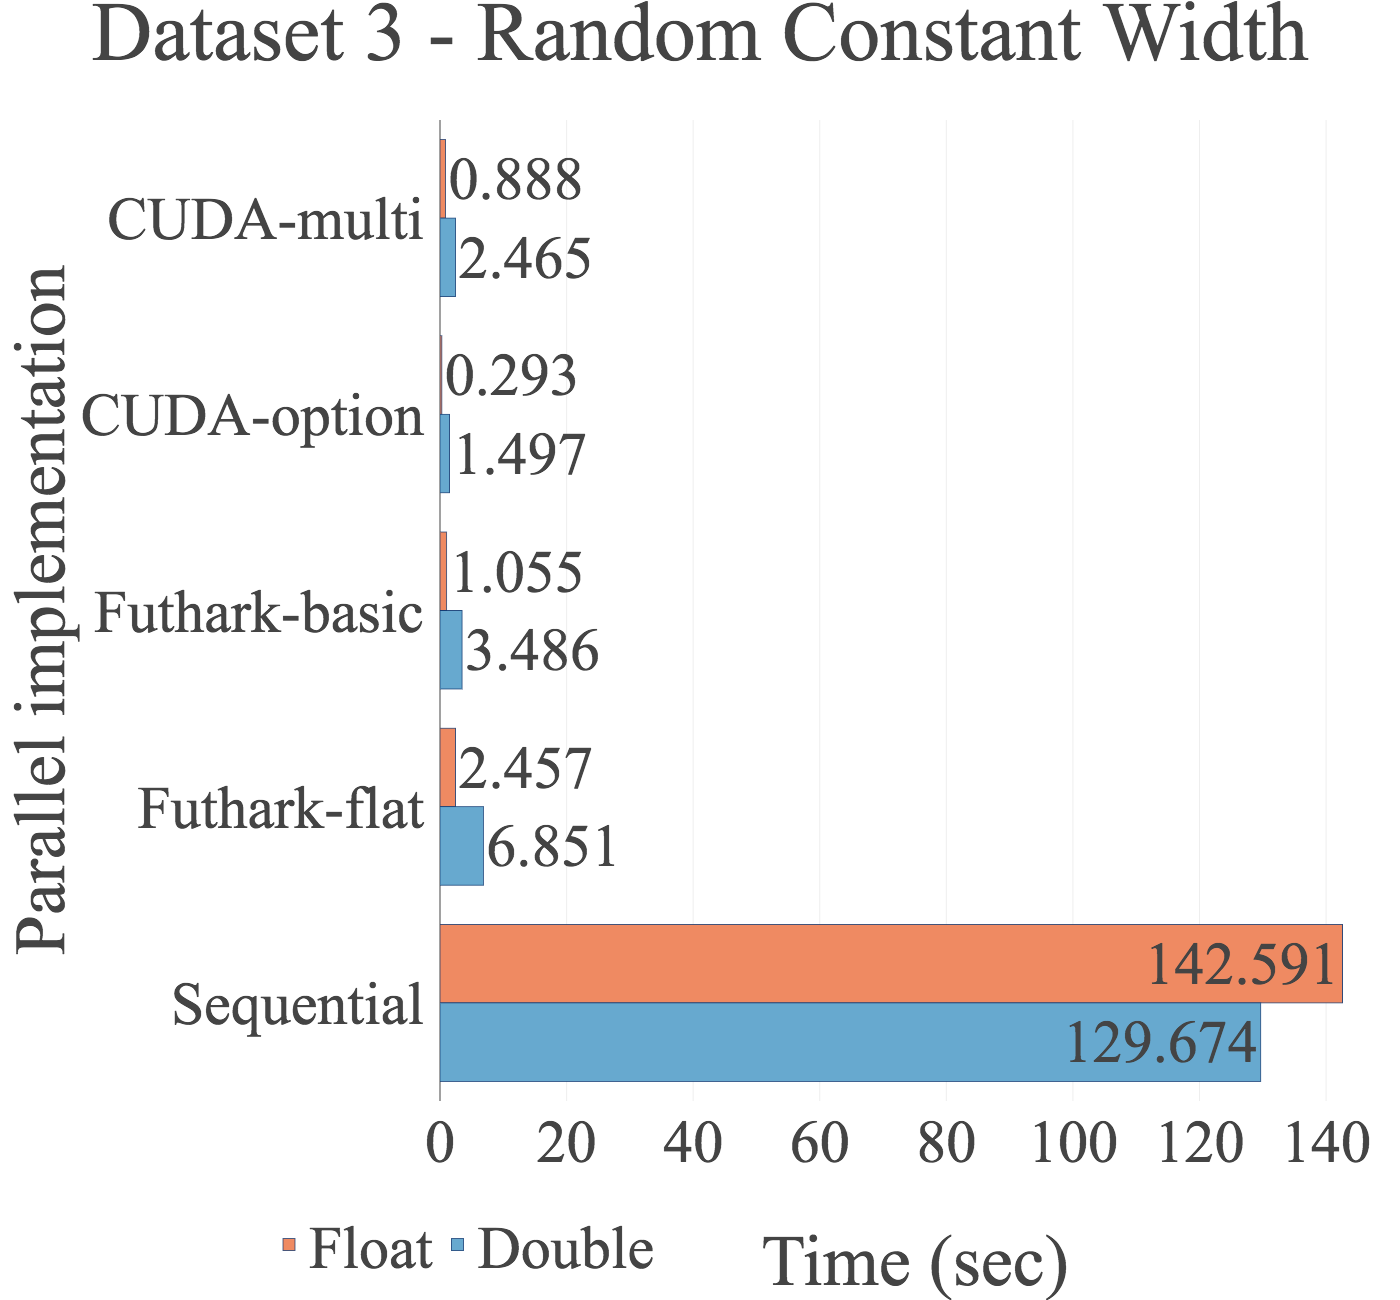
\includegraphics[width=1\textwidth]{img/experiments/all-approaches-3_RANDCONSTWIDTH.png}
\end{subfigure}
\end{adjustwidth}
\end{figure}

\begin{figure}[H]
\begin{adjustwidth}{-2cm}{-2cm}
\begin{subfigure}{.62\textwidth}
  \centering
  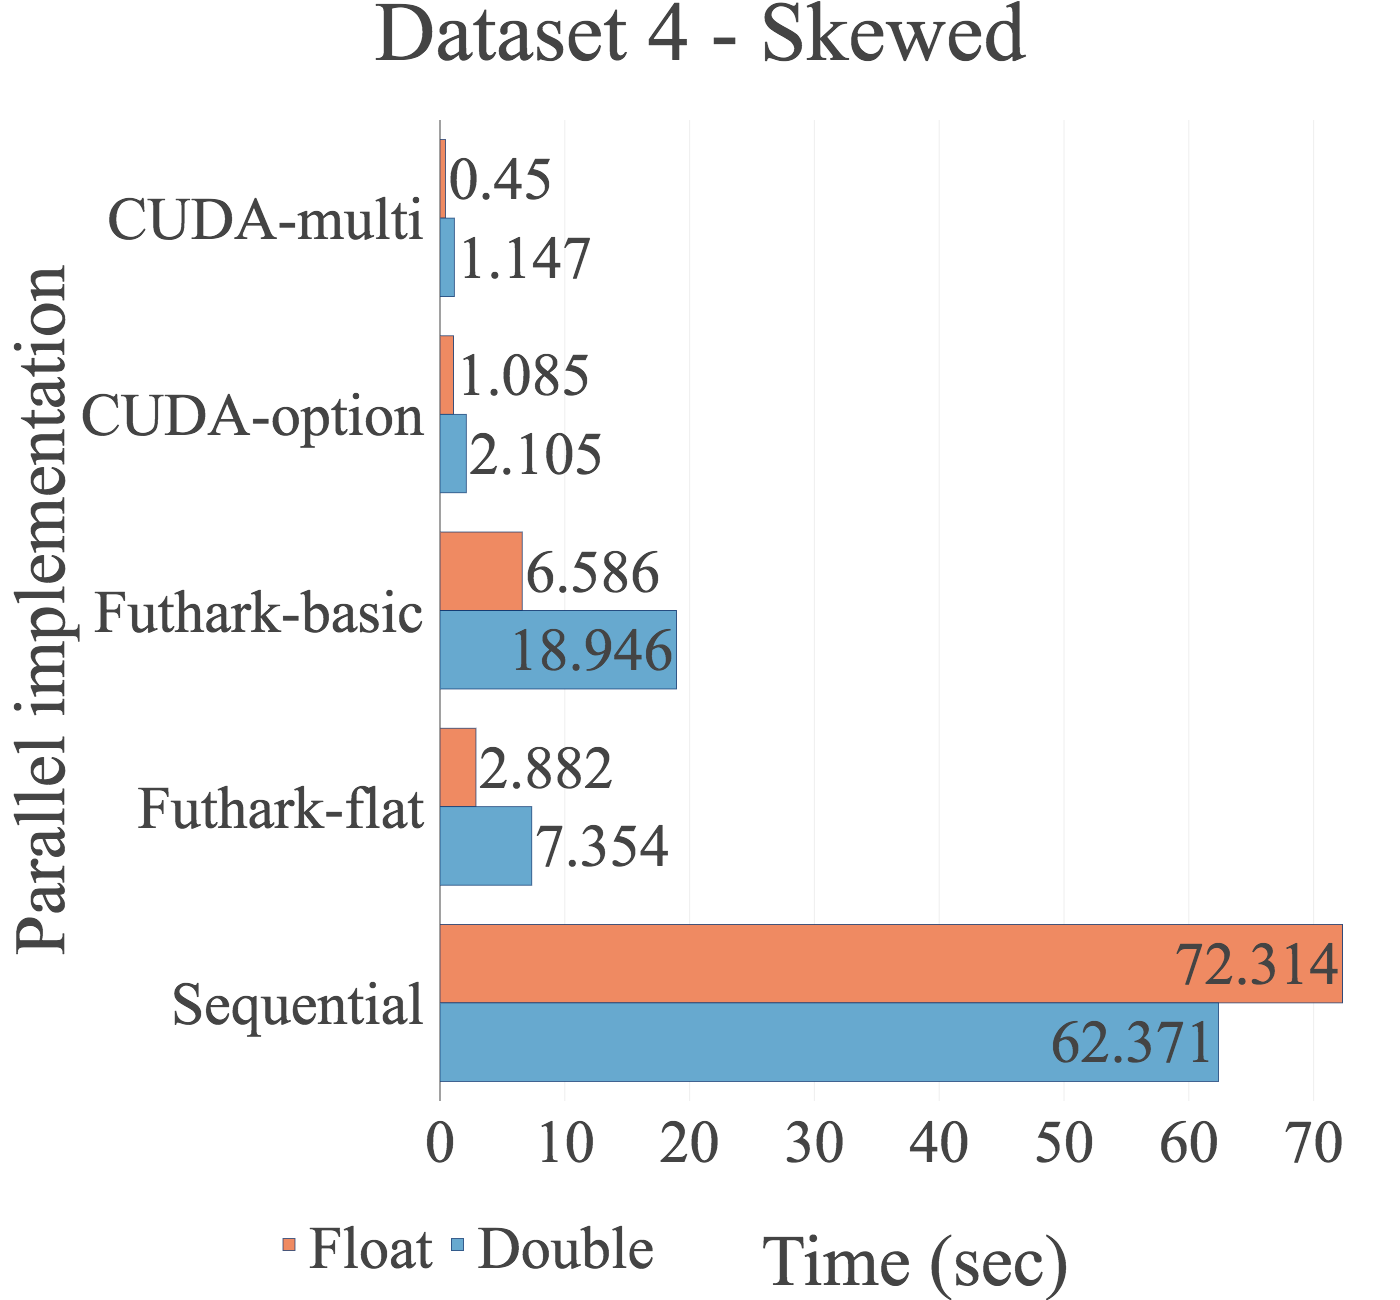
\includegraphics[width=1\textwidth]{img/experiments/all-approaches-4_SKEWED.png}
\end{subfigure}
\begin{subfigure}{.62\textwidth}
  \centering
  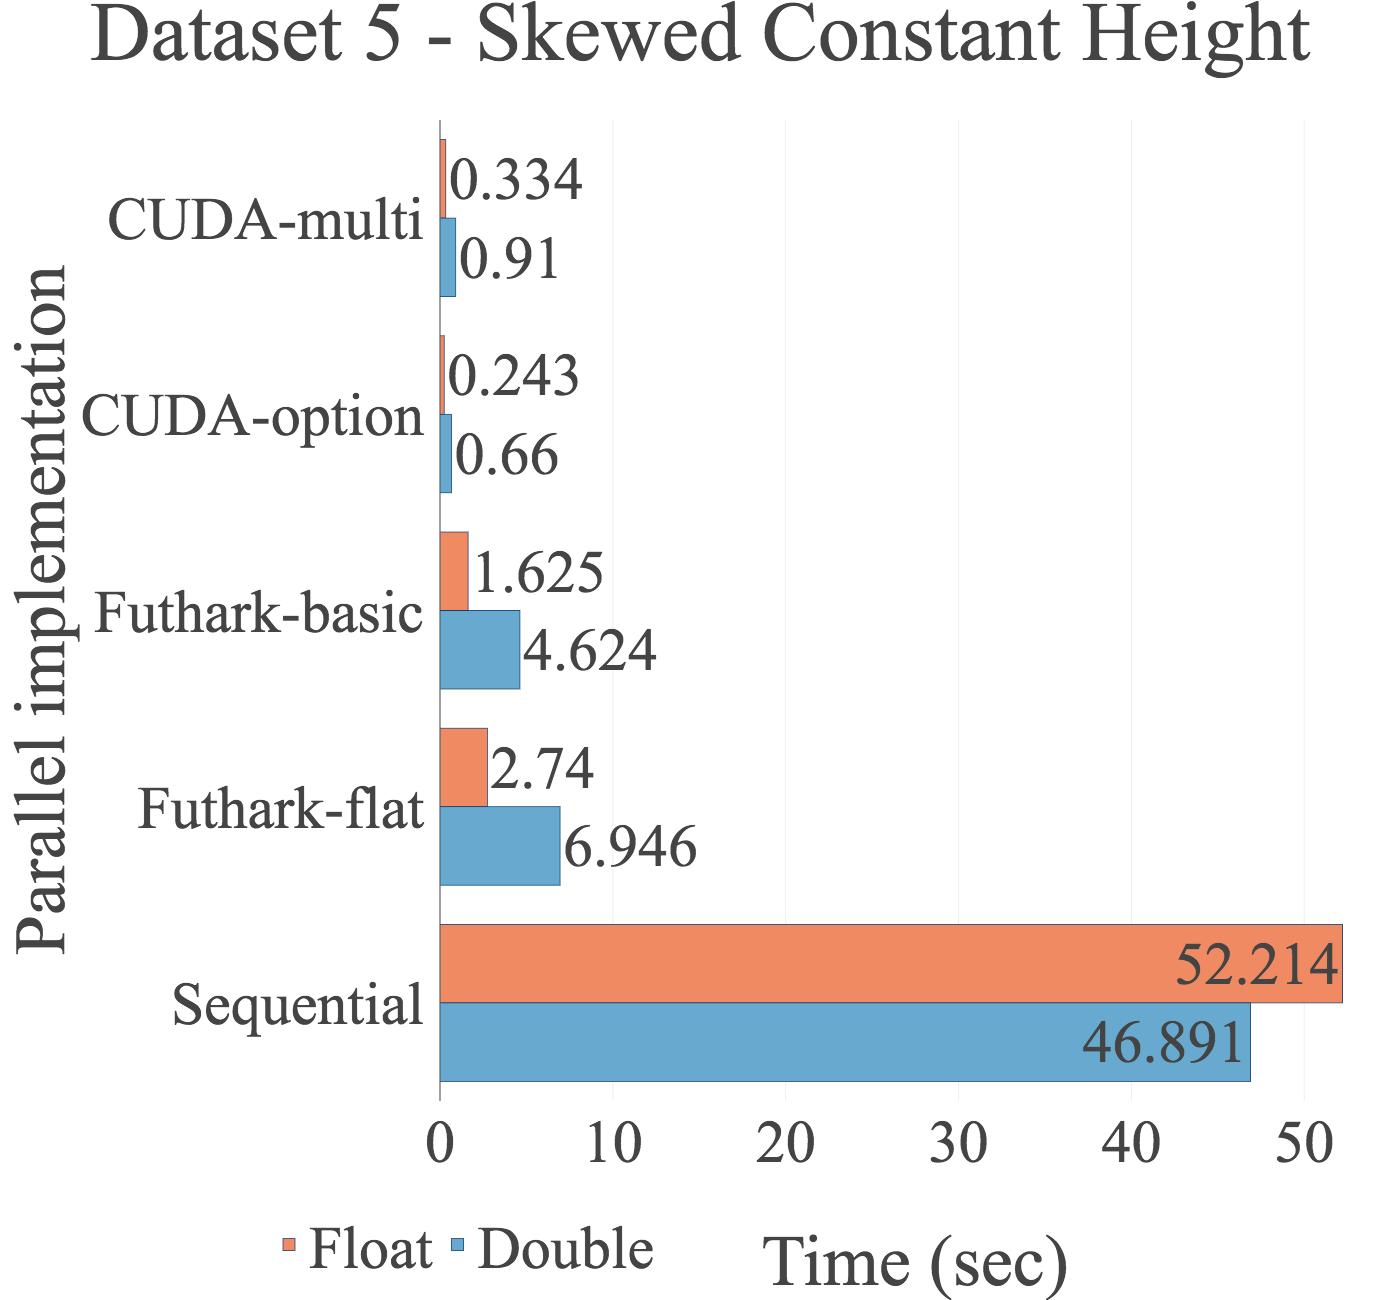
\includegraphics[width=1\textwidth]{img/experiments/all-approaches-5_SKEWEDCONSTHEIGHT.png}
\end{subfigure}
\par\bigskip
\par\bigskip
\centering
\begin{subfigure}{.62\textwidth}
  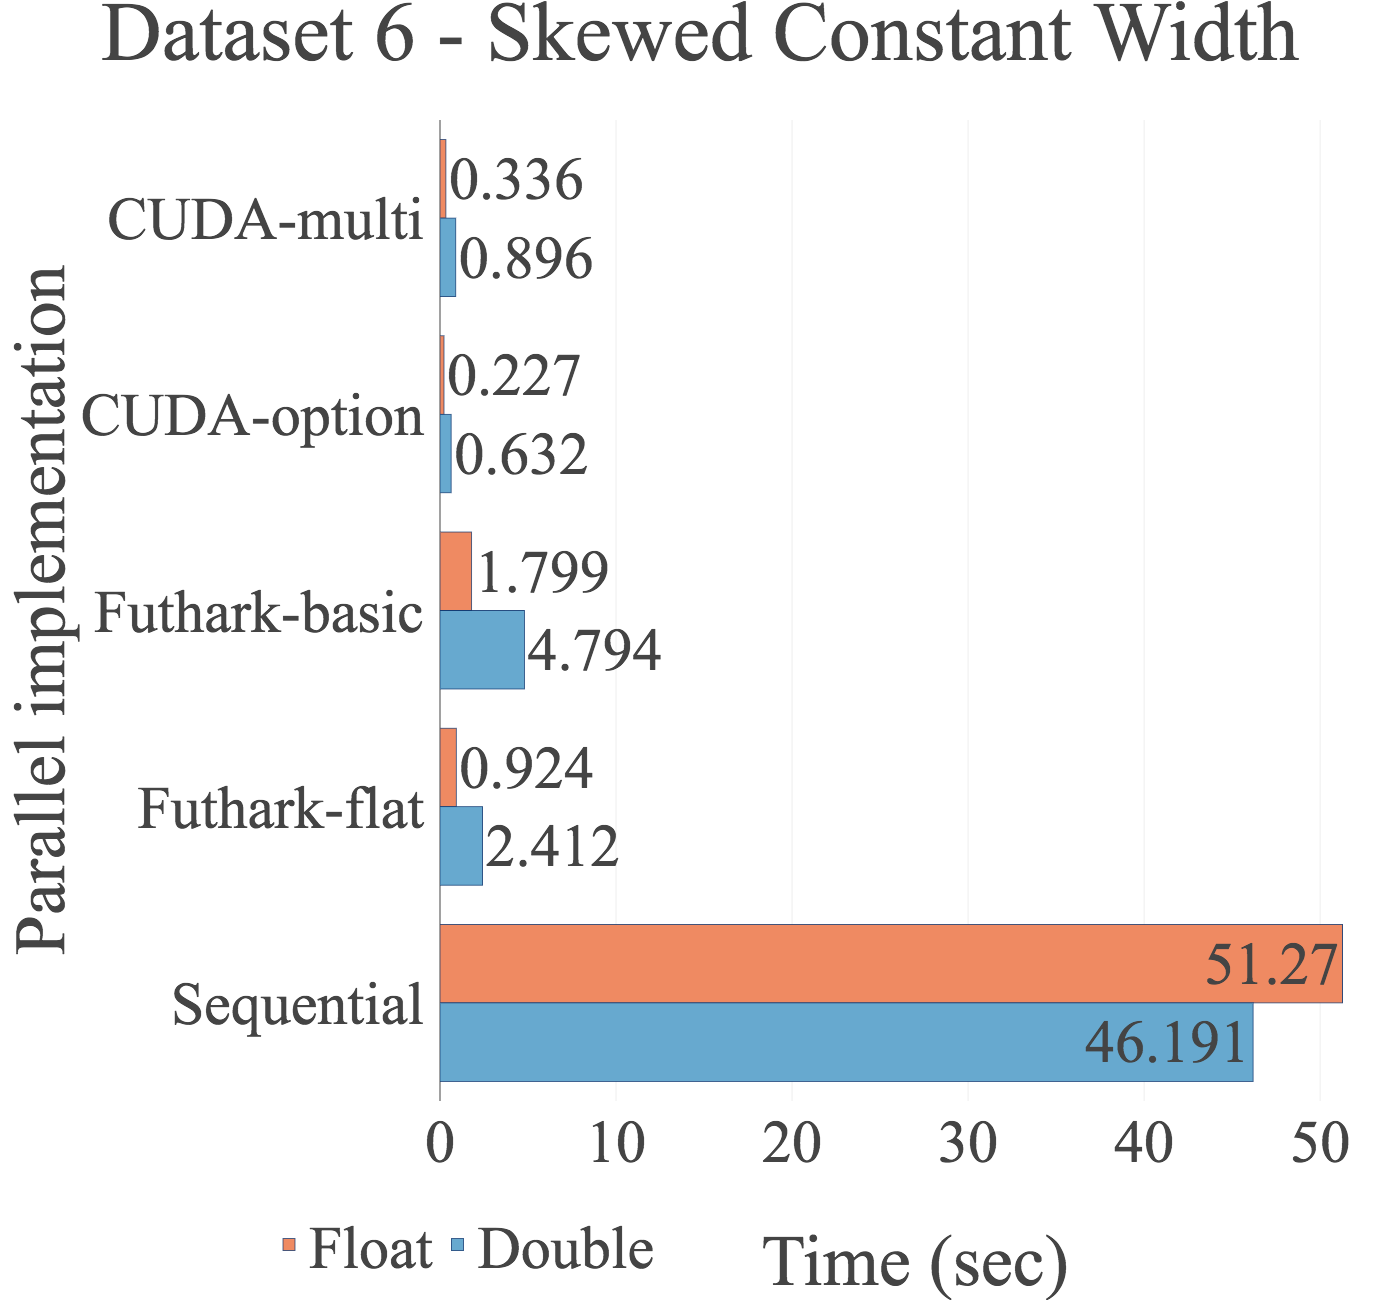
\includegraphics[width=1\textwidth]{img/experiments/all-approaches-6_SKEWEDCONSTWIDTH.png}
\end{subfigure}
\end{adjustwidth}
\end{figure}

% SECTION END %


\section{Speed-up on Small Datasets (Float)}
\begin{figure}[H]
\begin{adjustwidth}{-2cm}{-2cm}
	\centering
    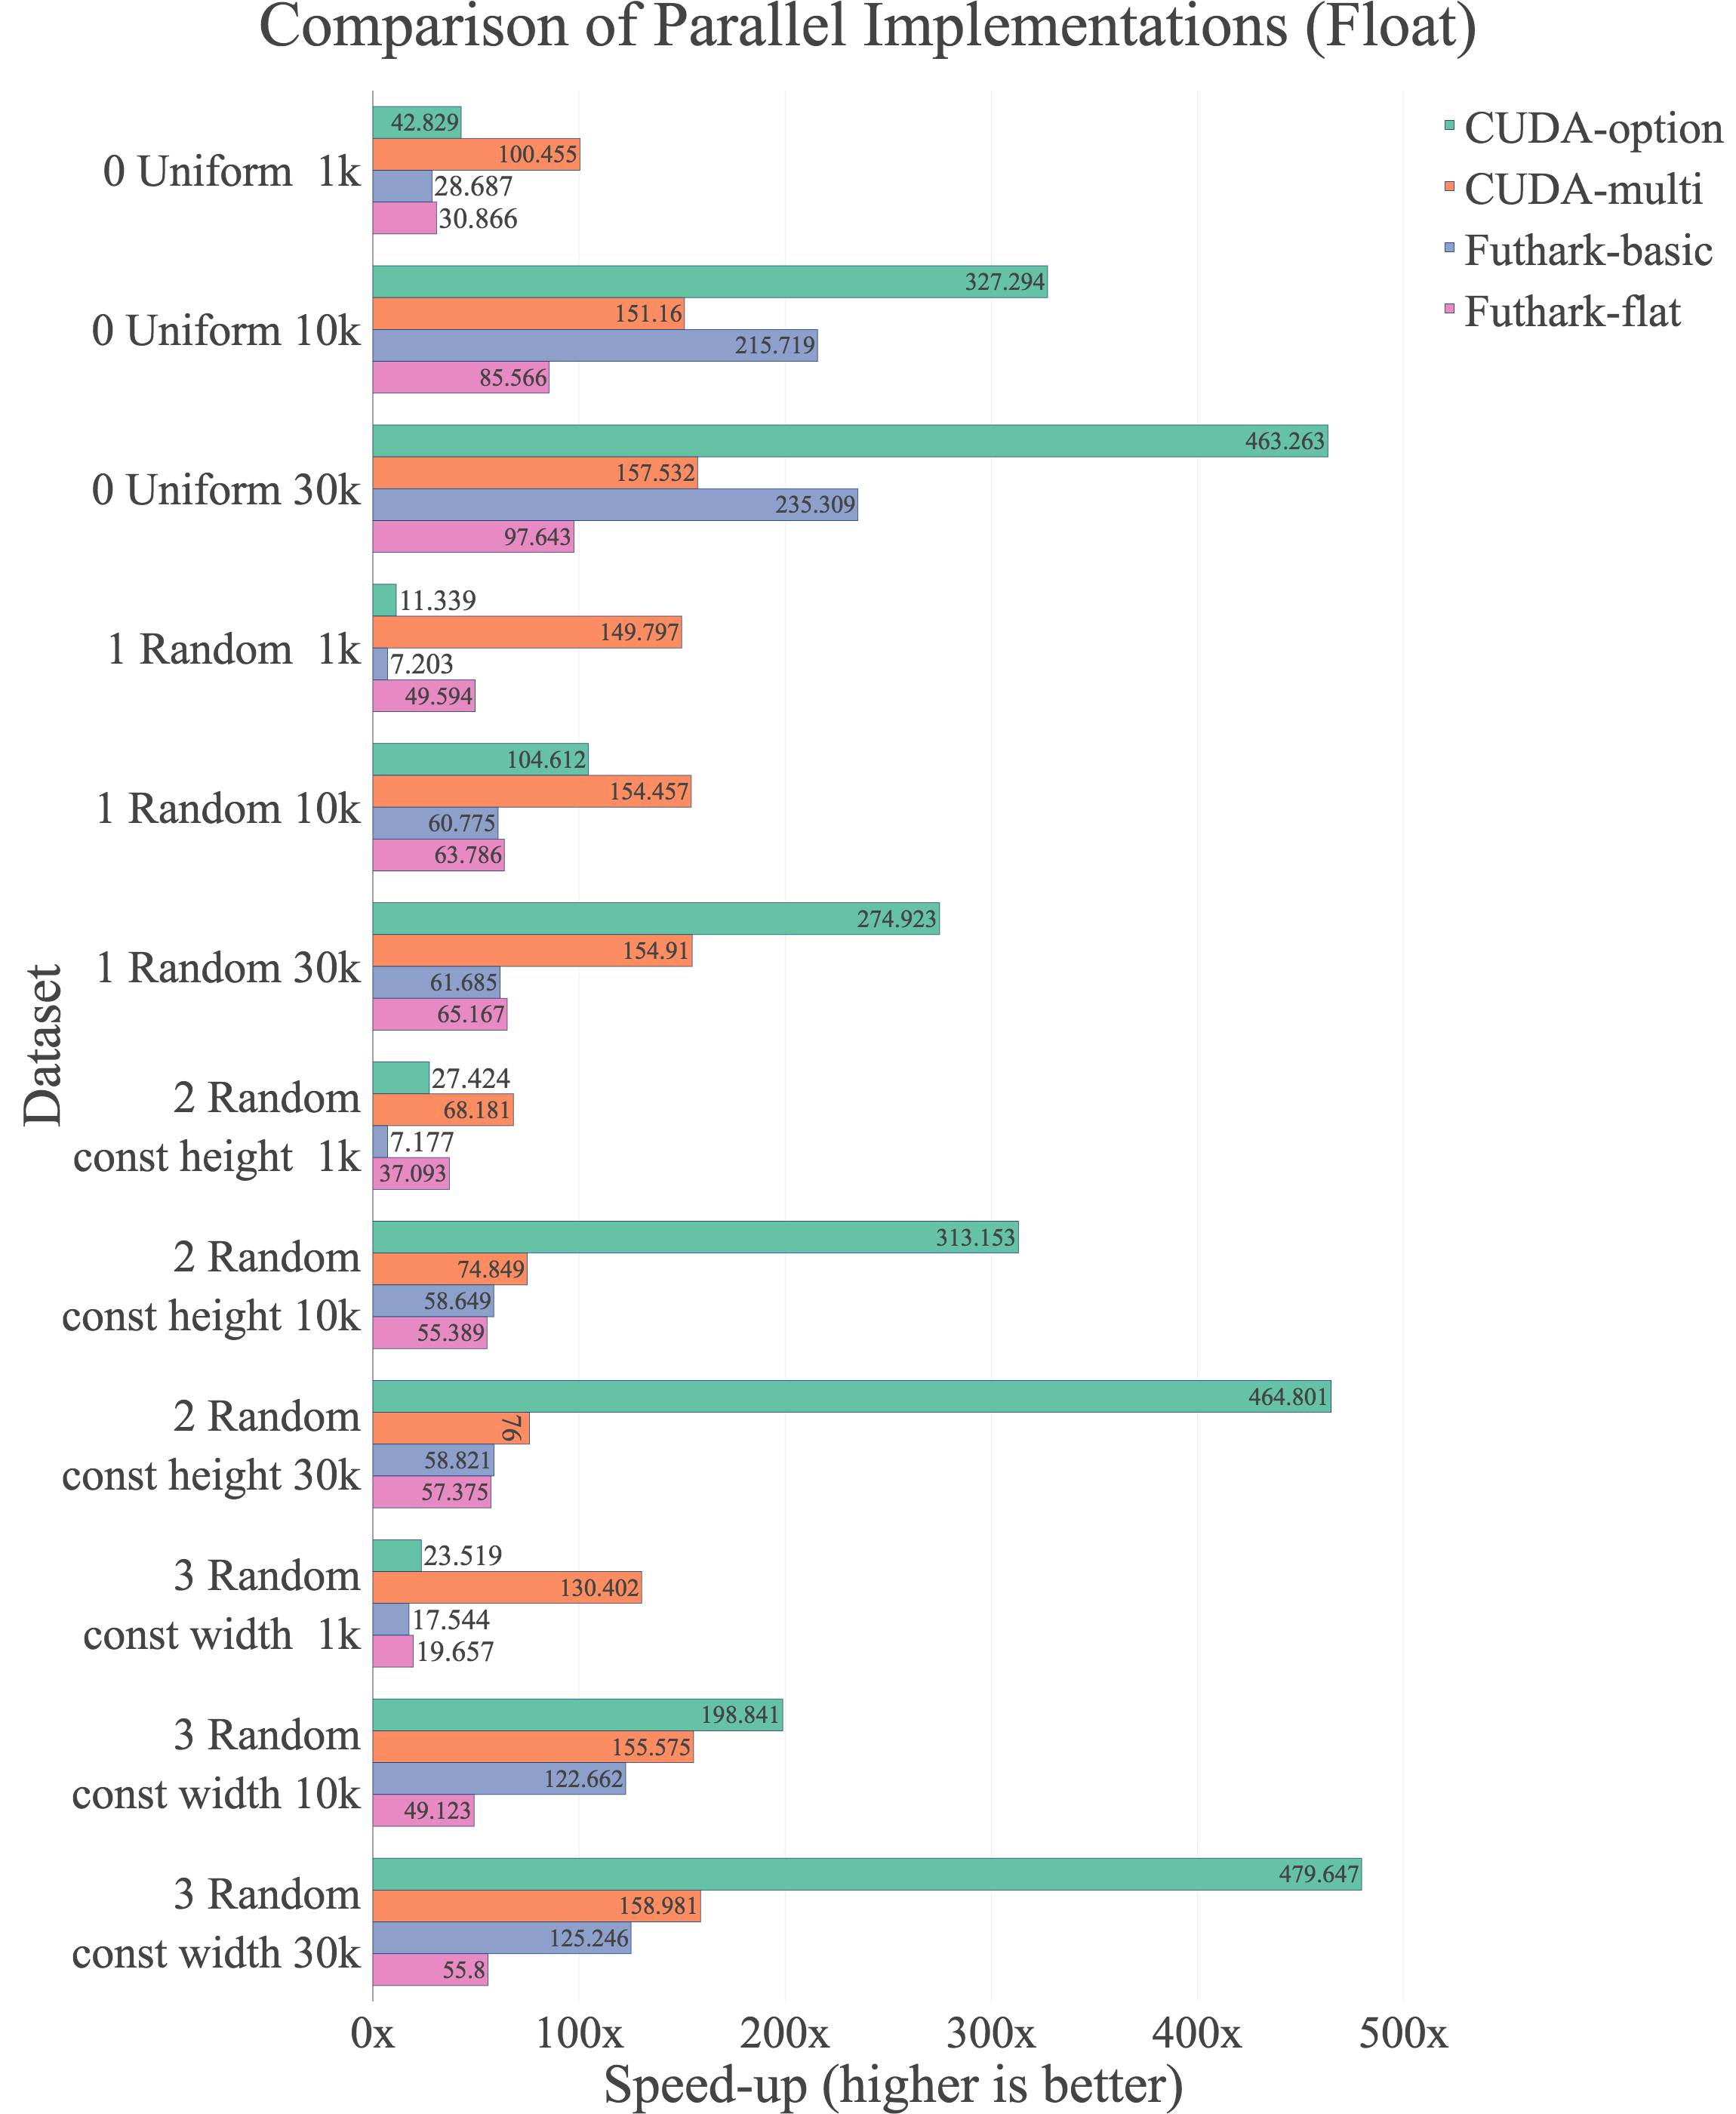
\includegraphics[width=1\textwidth]{img/experiments/small-all-approaches-float.png}
\end{adjustwidth}
\end{figure}

\section{Speed-up on Small Datasets (Double)}
\begin{figure}[H]
\begin{adjustwidth}{-2cm}{-2cm}
	\centering
    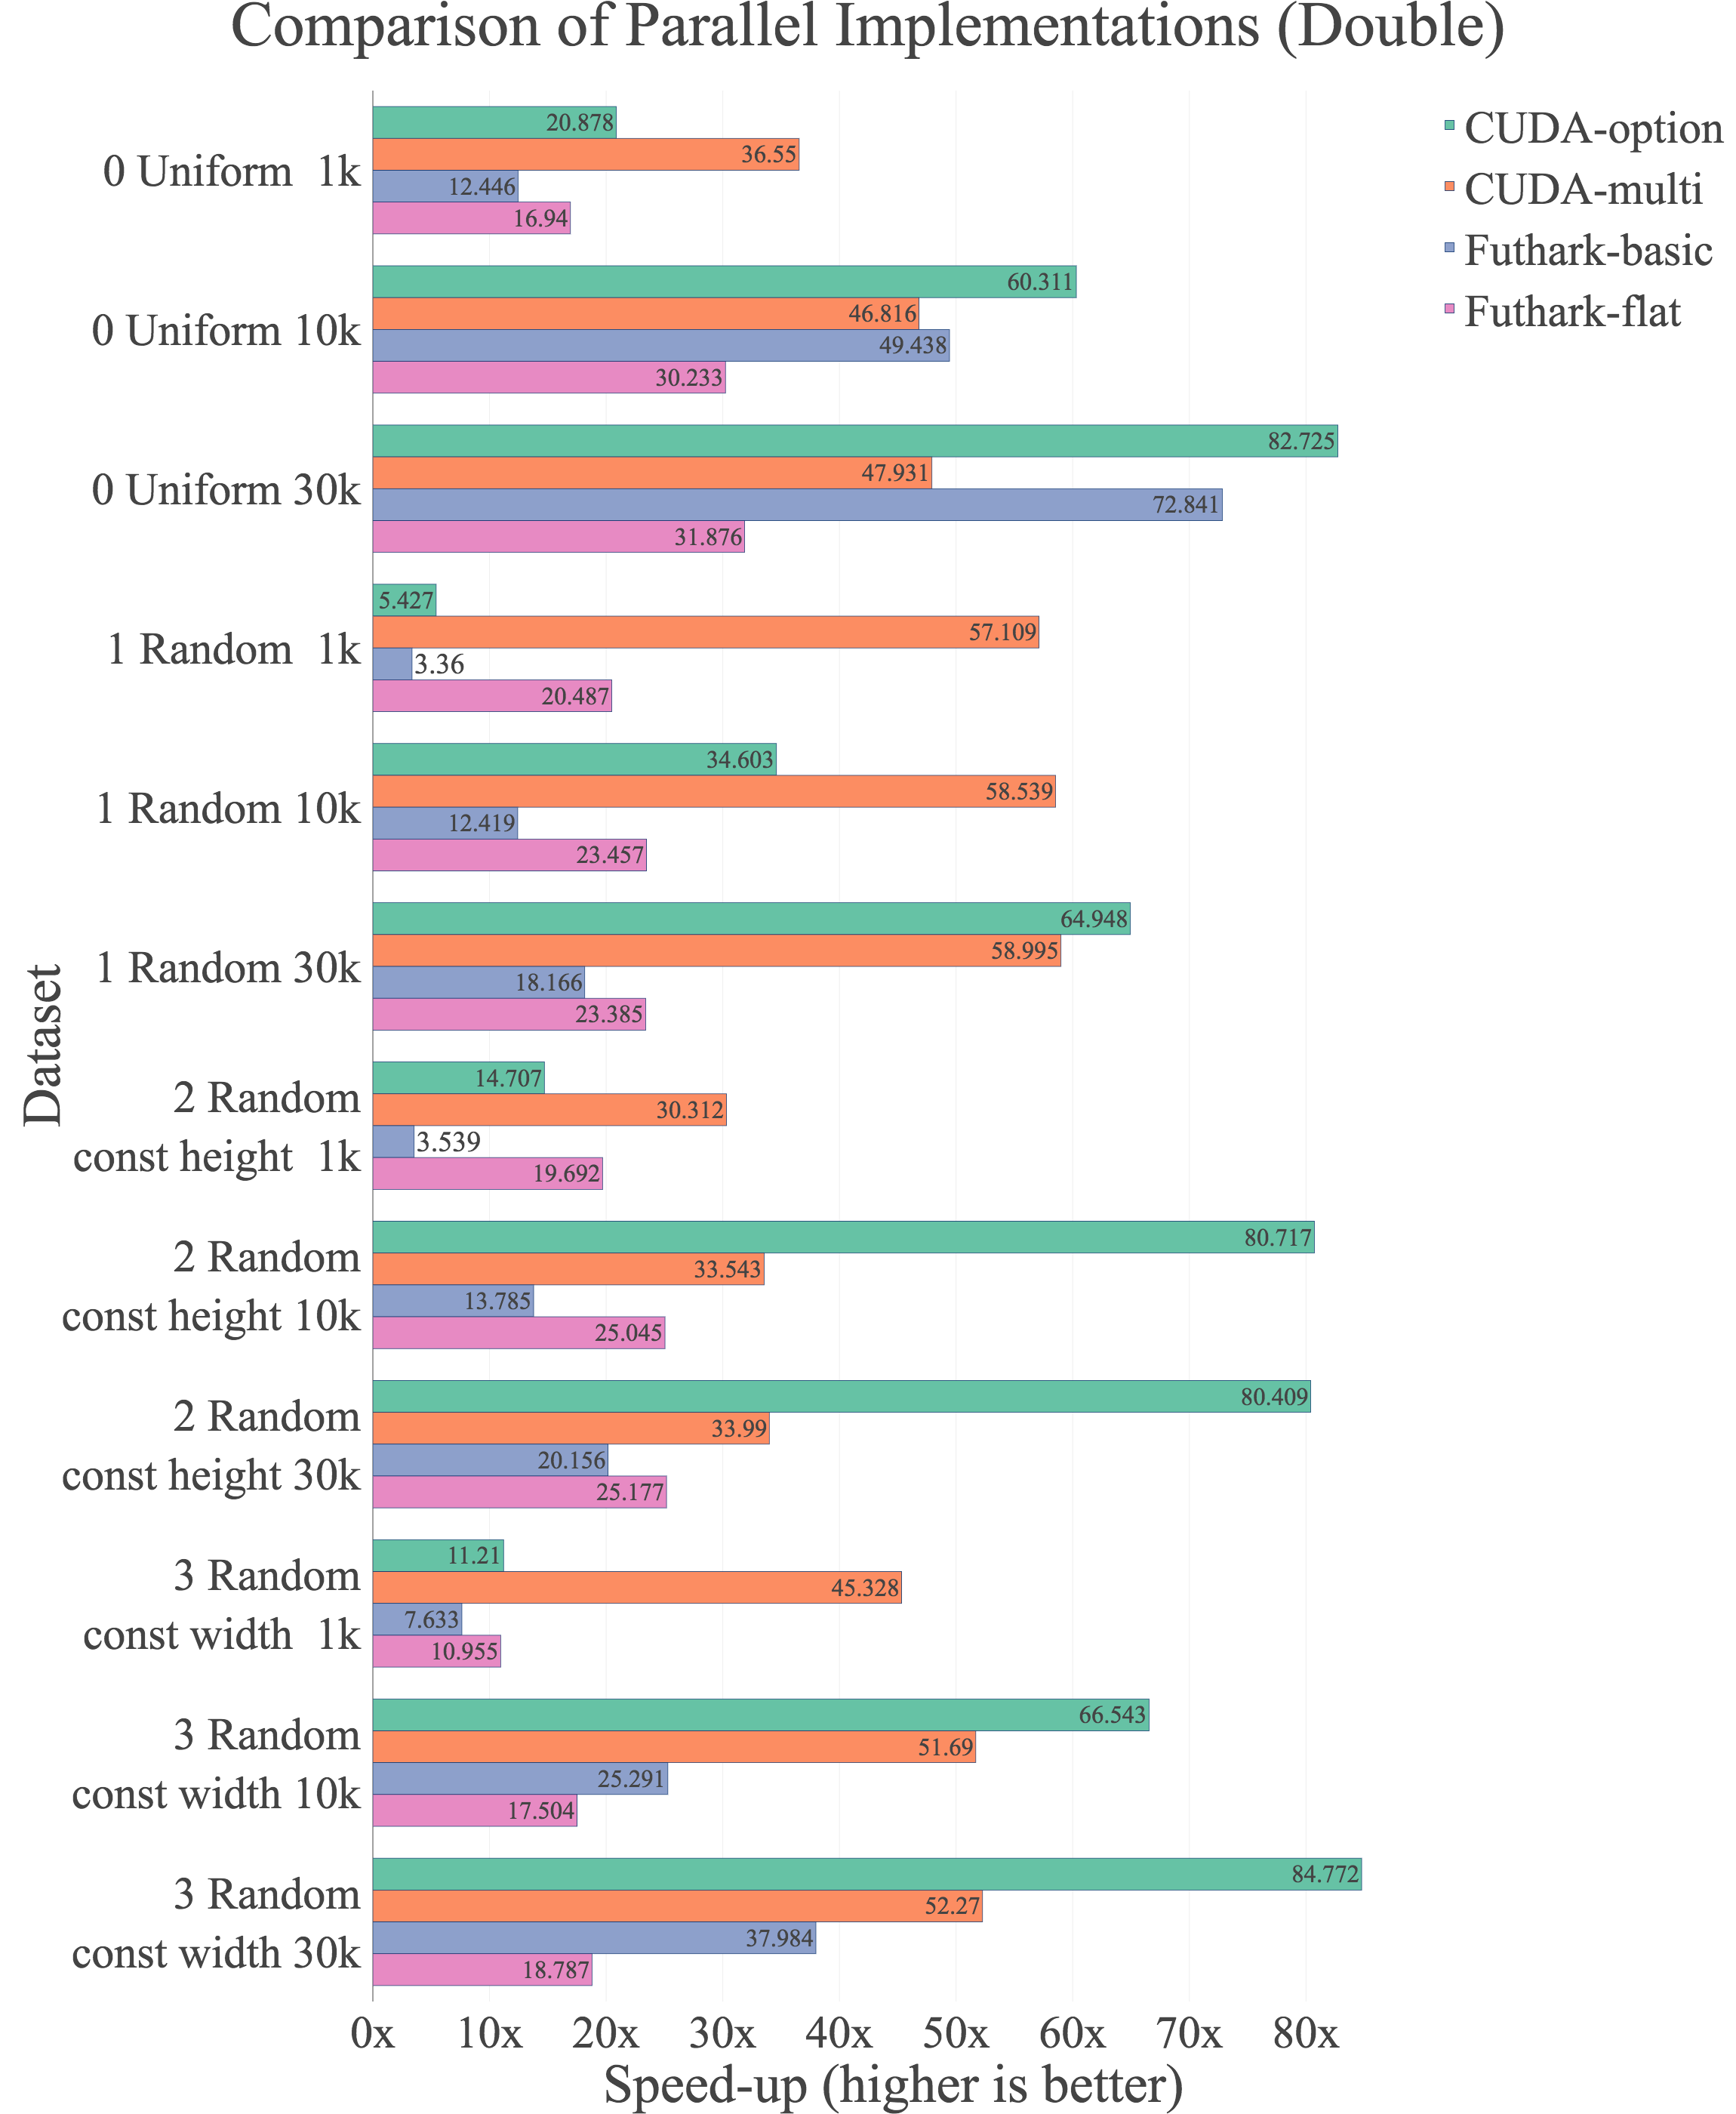
\includegraphics[width=1\textwidth]{img/experiments/small-all-approaches-double.png}
\end{adjustwidth}
\end{figure}